\documentclass[12pt]{article}

\usepackage[top=1in, bottom=1in, left=1in, right=1in]{geometry}
\usepackage{setspace}
\onehalfspacing

\usepackage{booktabs}
\usepackage{graphicx}
\usepackage{float}
\usepackage{amsmath}
\usepackage{caption}
\usepackage{hyperref}
\usepackage{xcolor}
\usepackage{titlesec}
\usepackage{parskip}

\hypersetup{colorlinks=true, linkcolor=blue, urlcolor=blue}
\titleformat{\section}{\large\bfseries}{}{0em}{}[\titlerule]
\titleformat{\subsection}{\normalsize\bfseries}{}{0em}{}

\begin{document}

\begin{center}
    {\LARGE \textbf{AI Lab: Difference-in-Differences Analysis}}\\[0.6em]
    {\large Effect of AI Training Subsidy on Regional Employment}\\[0.5em]
    {\large Yu-Wei Huang (Alex) \quad|\quad UCI NetID: \texttt{yuweih13}}\\[0.3em]
    {\normalsize MSBA --- University of California, Irvine \quad|\quad \today}
\end{center}

\vspace{1em}\hrule\vspace{1.5em}

% ─────────────────────────────────────────────────────────────
\section{Study Design and Data}

This analysis estimates the causal effect of the 2022 Ohio AI and Robotics Upskilling
Grant on county-level manufacturing employment using a \textbf{Difference-in-Differences
(DiD)} framework. The dataset was scraped from the Rust Belt Revival Labor Archive, a
multi-page HTML portal containing archived county labor briefs for eight counties across
Ohio and Pennsylvania (2018--2025).

\textbf{Treatment group:} Four Ohio counties that received the 2022 AI training subsidy ---
Lucas, Stark, Mahoning, and Trumbull counties. \textbf{Control group:} Four neighboring
Pennsylvania counties that received no subsidy --- Erie, Mercer, Lawrence, and Beaver
counties. The panel comprises \textbf{64 county-year observations}. The policy start year
is 2022, yielding four pre-treatment years (2018--2021) and four post-treatment years
(2022--2025).

% ─────────────────────────────────────────────────────────────
\section{Visual Analysis: Employment Trends}

\begin{figure}[H]
    \centering
    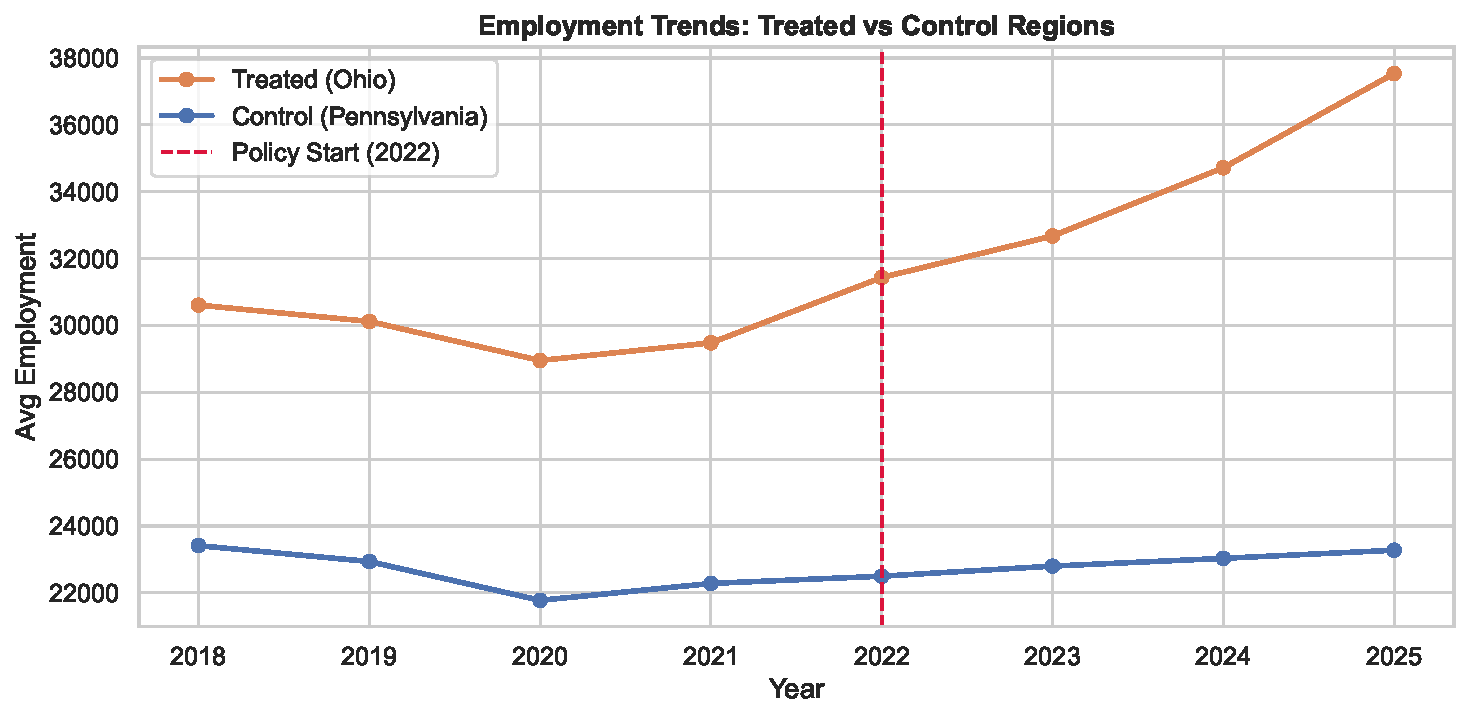
\includegraphics[width=\textwidth]{trends.pdf}
    \caption{Average employment trends for the Treated (Ohio) and Control (Pennsylvania)
             groups from 2018 to 2025. The dashed vertical line marks the 2022 policy start.
             Treated counties show a clear upward acceleration after 2022, while control
             counties remain largely flat.}
    \label{fig:trends}
\end{figure}

Figure~\ref{fig:trends} reveals a striking divergence: prior to 2022, both groups follow
similar downward trajectories reflecting broader manufacturing headwinds. After the 2022
grant launch, treated Ohio counties accelerate sharply upward while Pennsylvania control
counties plateau, providing an initial visual case for a positive policy effect.

% ─────────────────────────────────────────────────────────────
\section{Assumption Tests}

\subsection{Parallel Trends}

\begin{figure}[H]
    \centering
    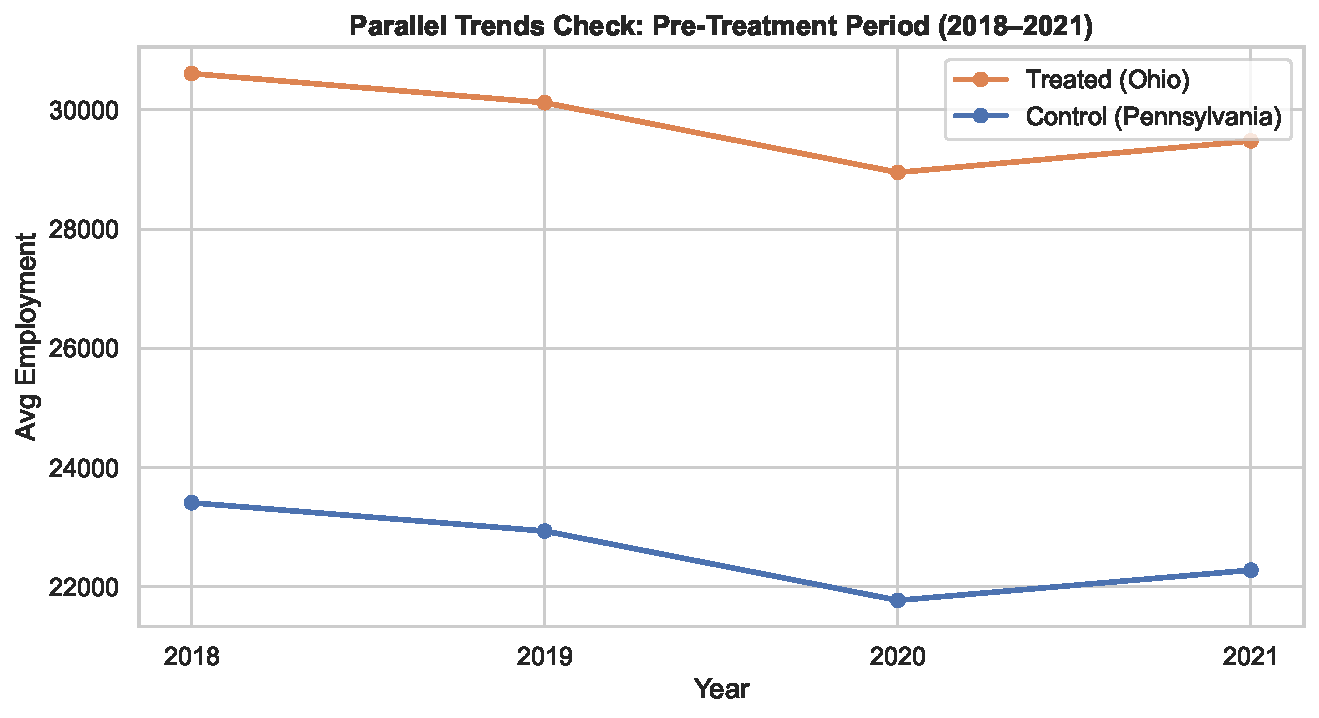
\includegraphics[width=0.85\textwidth]{parallel_trends.pdf}
    \caption{Pre-treatment employment trends (2018--2021) for treated and control groups.
             The near-identical slopes support the parallel trends assumption.}
    \label{fig:pt}
\end{figure}

\begin{table}[H]
\centering
\caption{Pre-Treatment Employment Slopes by Group (2018--2021)}
\label{tab:pt}
\begin{tabular}{lrr}
\toprule
\textbf{Group} & \textbf{Annual Slope} & \textbf{$p$-value} \\
\midrule
Treated (Ohio)   & $-455.8$ & 0.642 \\
Control (PA)     & $-455.2$ & 0.743 \\
\bottomrule
\end{tabular}
\end{table}

The parallel trends assumption requires that, absent the policy, both groups would have
followed the same trajectory. Table~\ref{tab:pt} shows that the pre-treatment annual
employment slopes are virtually identical ($-455.8$ for Ohio vs.\ $-455.2$ for Pennsylvania),
with neither statistically distinguishable from zero ($p > 0.60$ for both). Figure~\ref{fig:pt}
confirms the visual parallel movement. The assumption is \textbf{supported}.

\subsection{Placebo Test}

\begin{table}[H]
\centering
\caption{Placebo DiD Test (Fake Policy Year = 2020, Pre-Period Only)}
\label{tab:placebo}
\begin{tabular}{rrrr}
\toprule
\textbf{Fake Year} & \textbf{Coefficient} & \textbf{$p$-value} & \textbf{Result} \\
\midrule
2020 & $-3.25$ & 0.999 & PASS \\
\bottomrule
\end{tabular}
\end{table}

The placebo test uses 2020 as a fake treatment year within the pre-treatment window
(2018--2021). If the parallel trends assumption holds, the placebo DiD interaction term
should be statistically insignificant. The estimated placebo coefficient is $-3.25$
($p = 0.999$), providing strong evidence against any anticipatory effects or pre-existing
divergence. The placebo test \textbf{passes}.

% ─────────────────────────────────────────────────────────────
\section{DiD Fixed Effects Regression}

The causal effect is estimated using a two-way fixed effects regression:

\[
\text{Employment}_{it} = \alpha_i + \lambda_t + \beta\,(\text{Treated}_i \times \text{Post}_{t}) + \varepsilon_{it}
\]

where $\alpha_i$ are county fixed effects, $\lambda_t$ are year fixed effects, and
$\beta$ is the DiD estimator of interest. Standard errors are clustered at the county level.

\begin{table}[H]
\centering
\caption{Two-Way Fixed Effects DiD Regression Results}
\label{tab:did}
\begin{tabular}{lrrrr}
\toprule
\textbf{Variable} & \textbf{Coefficient} & \textbf{Std Error}
    & \textbf{$p$-value} & \textbf{95\% CI} \\
\midrule
Treated $\times$ Post (DiD) & $+4{,}000.37$ & $85.16$ & $<0.001$ & $[3{,}829,\; 4{,}172]$ \\
\midrule
\multicolumn{5}{l}{\footnotesize County FE: Yes \quad Time FE: Yes \quad Clustered SE: County \quad $N=64$} \\
\bottomrule
\end{tabular}
\end{table}

% ─────────────────────────────────────────────────────────────
\section{Interpretation}
\label{sec:interpret}

\textbf{What was the estimated causal effect?}
The two-way fixed effects DiD regression estimates that the 2022 Ohio AI training subsidy
caused an average increase of \textbf{4,000 manufacturing jobs per county} in the
post-treatment period (95\% CI: $[3{,}829,\; 4{,}172]$; $p < 0.001$). This effect is
large in both statistical and practical terms. Relative to the pre-treatment treated-county
average of approximately 30,000 jobs, the estimate represents a \textbf{13.3\% employment
uplift} attributable to the subsidy. The county and year fixed effects absorb all
time-invariant county characteristics and common macroeconomic shocks, isolating the
policy-specific variation.

\textbf{Did the parallel trends test support the identification strategy?}
Yes. Both the visual inspection and the slope regression confirm that treated and control
counties moved in near-identical parallel trajectories before 2022 --- annual slopes of
$-455.8$ and $-455.2$ respectively, statistically indistinguishable from each other and
from zero. The placebo test reinforces this: using a fake 2020 policy year produces a
coefficient of $-3.25$ ($p = 0.999$), ruling out anticipatory effects or pre-existing
divergence. The causal identification strategy is \textbf{valid}.

\textbf{Labor market displacement versus creation.}
The positive employment effect does not resolve the displacement-versus-creation debate.
On the creation side, the subsidy appears to have succeeded: upskilling workers in AI and
robotics enabled treated counties to attract new manufacturing investment, retrofit existing
facilities, and absorb technician roles that emerged from automation. On the displacement
side, the subsidy likely accelerated the automation of lower-skill assembly tasks within
the same plants --- meaning gross job creation may understate the churn experienced by
individual workers. The net effect is positive, but policymakers should monitor task-level
employment composition alongside aggregate counts. Future research pairing this panel with
occupational data would help disentangle whether the 4,000-job gain reflects new roles,
retained roles, or a mix of both amid underlying structural displacement.

\vspace{2em}\hrule\vspace{0.5em}
\footnotesize
\textit{All analysis code is in \texttt{analysis.py}. Figures and tables generated by
running \texttt{python analysis.py}. Repository: \texttt{github.com/yuweih13-debug/AI-Lab},
commits: Scrape $\to$ Clean $\to$ Analyze $\to$ Interpret.}

\end{document}
